\documentclass[english]{DESCARWINreport}

\usepackage{times}
\usepackage{helvet}
\usepackage{courier}
\usepackage{graphicx}
\usepackage{multirow}
%\usepackage[utf8]{inputenc}
\usepackage{algorithm}
\usepackage[noend]{algorithmic}
\usepackage{amsmath}
\usepackage{amsfonts}
\usepackage{amssymb}
\usepackage{array}
\usepackage{subfigure}
\usepackage{lscape}

%%%%%%%%%%%%%%%%%5 includepdf
\usepackage[final]{pdfpages}

\algsetup{indent=1.8em}
\renewcommand{\algorithmiccomment}[1]{// #1}
\newcommand{\pp}{planning tasks}
\newcommand{\PP}{planning task}
\newcommand{\dae}{{\em Divide-and-Evolve}}
\newcommand{\DAEI}{{\sc D\&E}}
\newcommand{\DAEII}{{\sc DaE2}}
\newcommand{\DAE}{{\sc DaE}}
\newcommand{\DAEX}{{\sc DaE$_{\text{X}}$}}
\newcommand{\DAEYAHSP}{{\sc DaE$_{\text{YAHSP}}$}}
\newcommand{\CPT}{{\sc CPT}}
\newcommand{\LPG}{{\sc LPG}}
\newcommand{\LAMA}{{\sc LAMA}}
\newcommand{\TFD}{{\sc TFD}}
\newcommand{\YAHSP}{{\sc YAHSP}}

\def\UU{{\mathbb{U}}}

%\title{DESCARWIN\\\bigskip {\em \LARGE The Marriage of Descartes and Darwin}\\\bigskip \bigskip \bigskip \bigskip \bigskip \bigskip \bigskip {\LARGE WP1: the \DAEX\ Planning System}}
\title{DESCARWIN\\\bigskip {\em \LARGE The Marriage of Descartes and Darwin}\\\vspace{8cm} 
{\LARGE D2.2\\
Experiments using off-line methods}}
\date{\today}
\laboratory{TRT - INRIA - ONERA}
\docref{62 441 217-179-1}

\revision{-}

\setlength{\parindent}{0cm}
\setlength{\parskip}{2ex plus 0.5ex minus 0.2ex}

\newcounter{hyp}
\setcounter{hyp}{1}
\newcommand{\hyp}{H\thehyp\stepcounter{hyp}}
\newcounter{defi}
\setcounter{defi}{1}
\newcommand{\defi}{D\thedefi\stepcounter{defi}}
\newcounter{con}
\setcounter{con}{1}
\newcommand{\con}{C\thecon\stepcounter{con}}

% Pour r�duire globalement l'espace entre les items d'une liste
% on peut �galement utiliser le bout de code suivant de M. Wooding
% Les param�tres utilis�s pour d�finir cette mise en page
% sont les suivants :
% \topsep espace vertical suppl�mentaire (ajoute � \parskip)
% 	ins�r� entre le texte pr�c�dant la liste et le 1er objet
% 	de la liste
% \partosep espace vertical suppl�mentaire ins�r� devant la liste
% 	si celle-ci est pr�c�d�e d'une ligne blanche
% \itemsep espace vertical suppl�mentaire (ajout� � \parsep)
% 	ins�r� entre les �l�ments d'une liste.

%%%% debut macro %%%%
% \makeatletter
% \toks@\expandafter{\@listI}
% \edef\@listI{\the\toks@\setlength{\parsep}{0pt}}
% \edef\@listI{\the\toks@\setlength{\topsep}{0pt}}
% \makeatother
%%%% fin macro %%%%


\begin{document}

\maketitle

%\cleardoublepage

\begin{revisions}
\begin{revtable}
\dates{APR. 13, 2011}{}{}{}
\writers{Jacques Biba\"i\\Matthias Brendel\\Pierre Sav�ant\\Marc Schoenauer\\Vincent Vidal}{}{}{}
\approvers{P. Sav\'eant}{}{}{}
\end{revtable}
\begin{revisionlabels}
\revlabel{initial version}
\revlabel{}
\end{revisionlabels}
\end{revisions}

\begin{abstract}
This document reports experiments regarding the off-line tuning of the parameters of the Divide-and-Evolve method. Two very different approaches have been used, and for each one, a published paper presenting the corresponding work is included in this document after a short presentation.
\begin{itemize}
 \item The first Chapter presents work involving a standard {\em Racing} parameter tuning method, as introduced by Birratari et al. (reference [7] in the first paper). The goal is to find the best parameter setting for a class of instances, based on trials on a few instances for that class. The corresponding paper is ``On the Generality of Parameter Tuning in Evolutionary Planning'', by Jacques Biba�, Pierre Sav�ant, Marc Schoenauer, and Vincent Vidal, and was presented at the ACM-GECCO conference in July 2010 in Seattle (pp 241-248 of the proceedings).


\item The second Chapter introduces an original method for instance-based parameter tuning, where a model of difficulty w.r.t. given algorithm is learned on some sample instances, and used thereafter on unknown instances to predict which are the best parameters for this instance. The corresponding paper has been accepted for poster presentation at the ACM-GECCO 2011 in Dublin next July (proceedings not yet available).
\end{itemize}

\end{abstract}

\tableofcontents

% \newpage
% 
% \chapter{Introduction}

\newpage
\chapter{On the Generality of Parameter Tuning in Evolutionary Planning}
The paper presented in this Chapter presents off-line parameter tuning applied to DaE using the well-known Racing method [7]\footnote{The citations refer to the references of the following paper.}. The goal of the Racing method is to find the best setting of parameters among a finite pre-defined set of possible parameter settings. The brute force way would be to run the several instances of the algorithm with all available settings, and to use standard statistical analysis (e.g. ANOVA) to find out the best setting. The idea of Racing is to start running only a small number of runs per available setting, and to eliminate as early as possible the settings that obviously perform poorly (according to some statistical test). The process stop when either only one parameter setting remains, or when a pre-defined number of runs have been run for all settings - and standard ANOVA can then be used on the remaining settings. Typical savings compared to the brute force are from 50\% to 90\% of computational effort.

The other issue that arises when dealing with programs like DaE that optimize instances of a given problem is that of the generality of parameter tuning. The best results are of course obtained when the parameters are tuned anew for each instance that is to be optimized. However, this process is very costly indeed: even when using Racing, one parameter tuning process means represents several hundreds of complete runs. Hence the goal of parameter tuning in this situation is to find some parameter settings that give quasi-optimal results for several instances, or classes of instances. The closer the instances, the higher the chances that this is possible. Hence good candidates for such classes where all instances share some characteristics are the problem domains as defined in the IPC competitions: each domain contains around 30 instances that share the same objects types and actions. Picking up a few instances per domain, and running the Racing based on those instances only  hopefully results in parameter settings that generalize to the whole domain.
Finally, the ideal parameter setting should perform quasi-optimally on all instances of all domains. Similarly to what can be done within a domain, Racing is then done based on the results of the parameter sets on several instances of several domains.

The following paper contains the analysis of the results of the different options (tuning per instance, tuning per domain, global tuning). As expected, the more global the tuning, the worse the results. However, the results of the global tuning, frozen as the default parameter setting for DaE, allowed us to generate the comparative results of DaE with the state-of-the-art planners published in [4] that received the Silver Medal at the {\em Human Competitive Results} at ACM-GECCO conference in 2010.


\newpage
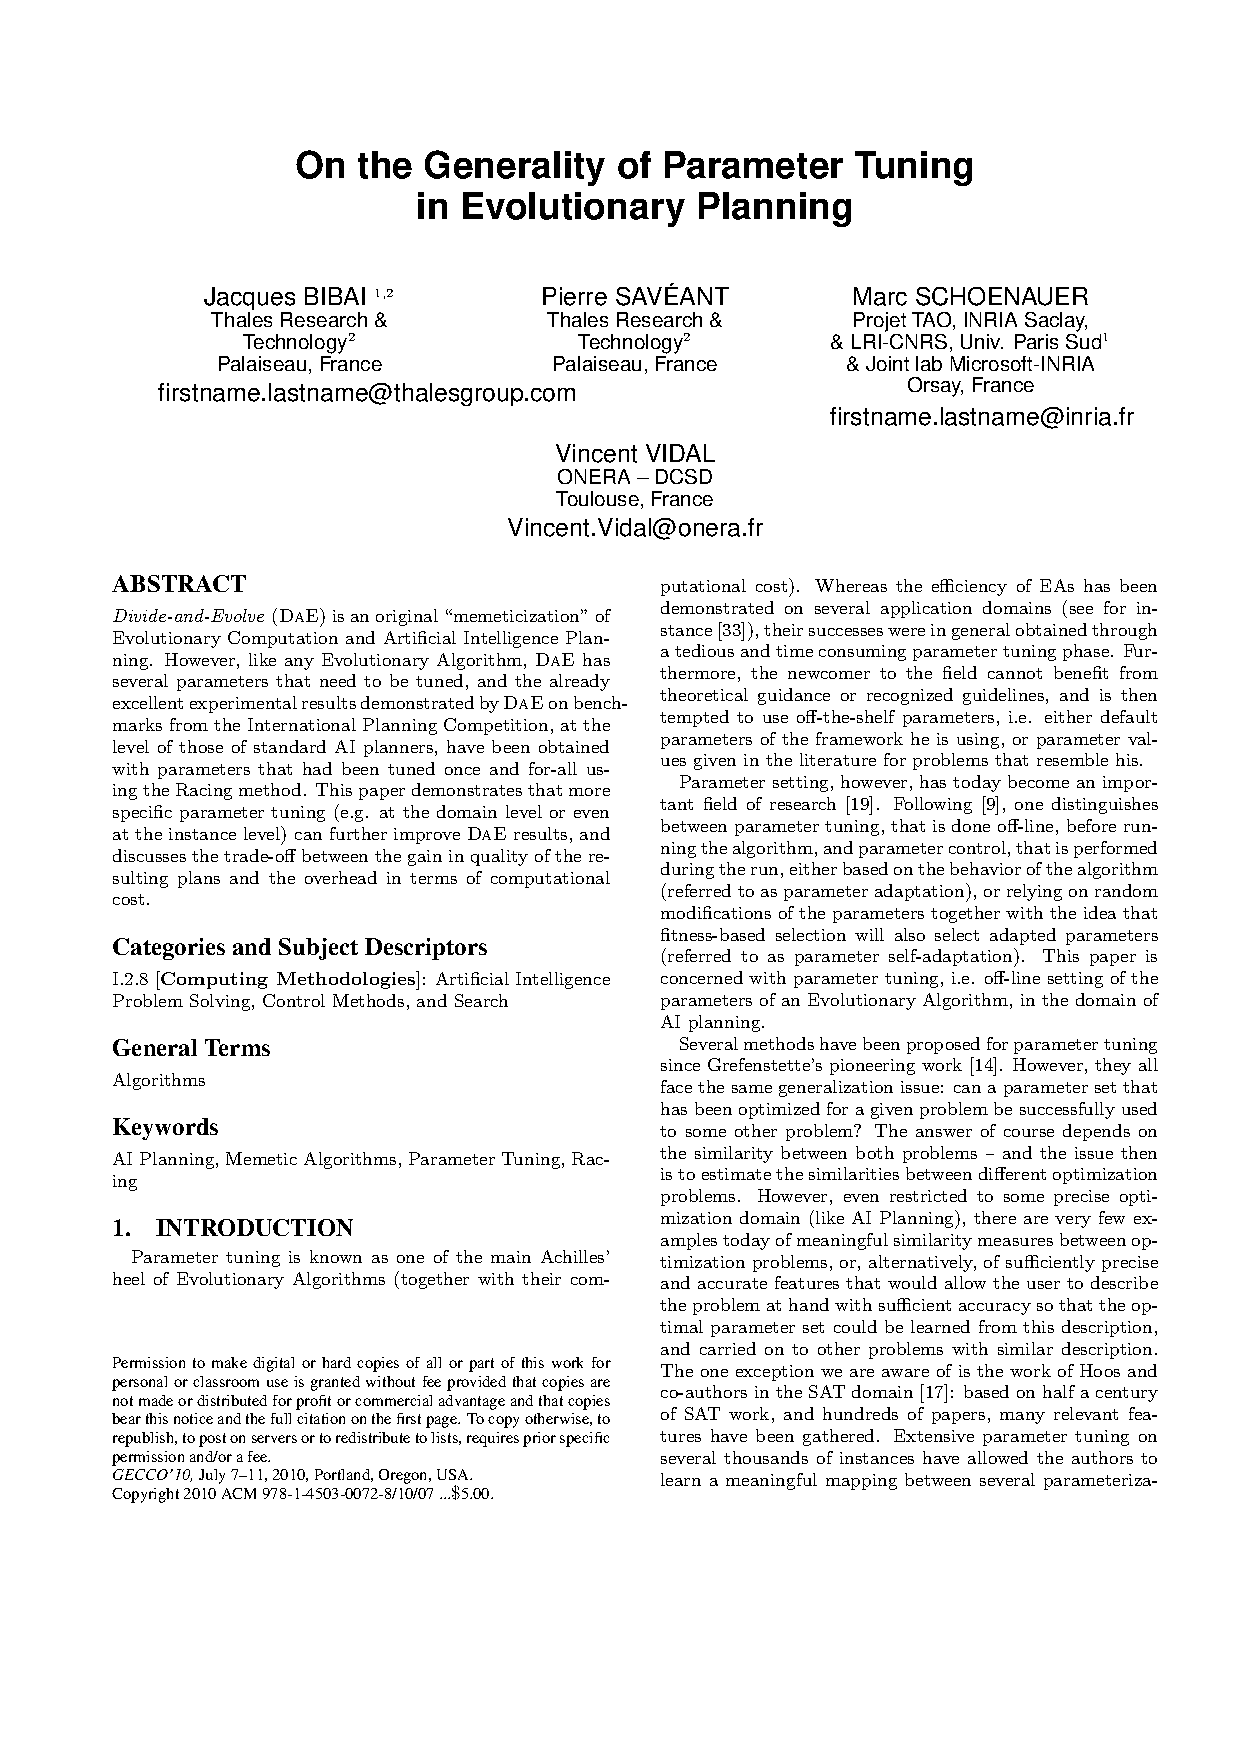
\includepdf[height=32cm,pages=-,offset=2.2cm -4cm]{gecco10.pdf}
\newpage
\chapter{Instance-Based Parameter Tuning for Evolutionary AI Planning}
The following paper presents the preliminary results of an original framework for instance-based off-line parameter tuning based on an empirical model of instance hardness that is learned from previous runs. Note that this framework could be used in other contexts than DaE. 
First examples of similar approach dates back to the work of Hutter et al. [13]\footnote{The citations refer to the references of the following paper.}, for SAT problems: instances are described by some features, and extensive experiments are run on many instances with many different solvers (or many different parameterizations of some solvers), and the performance of each solver on each instance is recorded. Machine Learning is then used to learn the mapping from (instance,solver) to performance. When a new instance is to be handled, the best solver is determined from the learned mapping, i.e., the one that should give the best performance according to the learned mapping.\\
There are three main issues when attempting to use such method on a new type of problem.
\begin{itemize}
 \item The design of the features that will be used to describe each instance of the problem. They should be discriminant enough so as to separate instances on which some algorithm behave differently. For the SAT domain [13], several dozens of features had been proposed in the literature, out of which 45 were chosen. No such features exist in the AI Planning area, and the preliminary work presented here is based on 14 elementary features gathered from statistics on the instance after the initial {\em grounding} step.

\item The choice of the performance that will be the output of the predictive model. For SAT problems, because only satisfiable problems were considered in [13], a natural performance is the time to solution. However, in the AI Planning domain, there is in general no known solution - and in any case, many algorithms or parameter setting never reach this optimal solution. Also, it is very difficult to set some general target such as ``reach the best makespan up to $\alpha$\%'' because there is no possible normalization of the makespans across instances. So another point of view had to be adopted, and the performance is computed the way it has been proposed in the IPC competitions (see e.g., [16] for a detailed description). Such performance was designed to allow a sound aggregation of the results across different instances.

\item The choice of the sample instances on which the model will be learned. This issue has already been discussed in the first paper presented in this document: the more instances the better, from a generalization point of view. But the more instances the higher the computational cost, and some trade-off had to be used.
\end{itemize}

Another issue regards the choice of the Machine Learning tool: Feed-forward Artificial Neural Networks with standard backpropagation algorithms are used here, though many other paradigms could have been used, and the results would probably have been similar.\\

However, there are two main novelties in the {\em Learn-and-Optimize} method proposed here: 
\begin{itemize}
\item First, the kind of mapping that is learned is not the (instance, parameters) to performance mapping, but directly the mapping from instance to optimal parameters. 

\item Second, the learning and optimization phases are intertwined: whereas in [13] all runs were run at once, and learning was achived in a single pass over the whole set of examples, the learning and optimization steps are much more intertwined in the LaO approach.

\end{itemize}

The preliminary results presented in the following are promising, and on-going work is concerned with addressing the first issue above -- the design of sound features -- as well as validaring the proposed approach on larger sets of instances.

\newpage
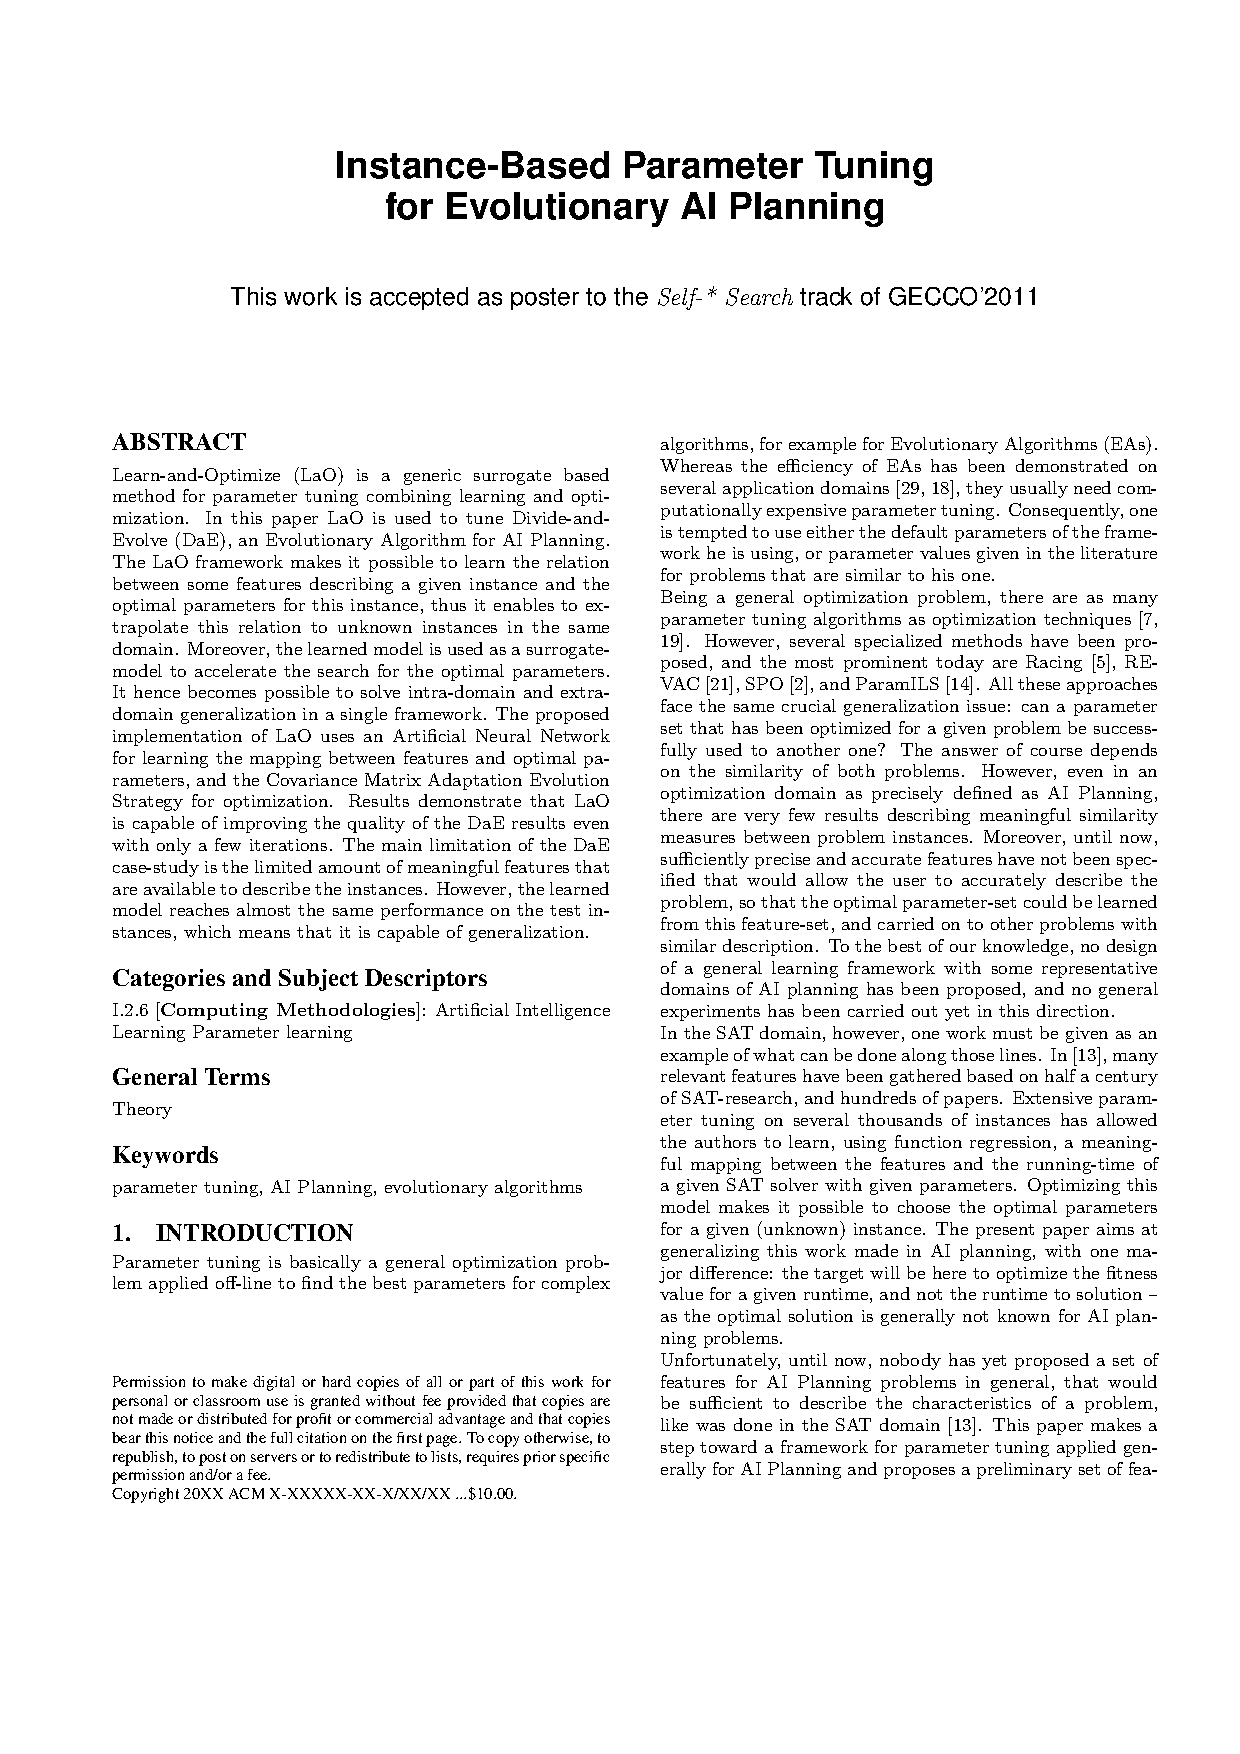
\includepdf[height=32cm,pages=-,offset=2.2cm -4cm]{gecco2011brendelschoenauer.pdf}

% \chapter{Conclusion}
% \label{conclusion}


% \chapter{References}
% \bibliographystyle{alpha}
% \bibliography{xxx}

\end{document}